\documentclass{cours}
\usepackage{esvect}
\usepackage{pgfplots}
\usepackage{multicol}
\usepackage{mathrsfs}
\usepackage{amssymb}
\usepackage{tikz-3dplot}
\usepackage{xr}
\usepackage{fontawesome}
\usetikzlibrary {decorations.text, backgrounds, intersections}

\begin{document}

\setcounter{chapter}{24}
\chapter{Lois de l'induction}
\section{Flux d'un champ magnétique}%
\label{sec:flux_d_un_champ_magnetique}

\subsection{Surface orientée}%
\label{sub:surface_orientee}

Soit une surface $S$, choisir une orientation de $S$, c'est choisir l'un des deux vecteurs unitaires directeurs de la normale à la surface. En général\footnote{Toutes les surfaces ne sont pas forcément orientables, par exemple un anneau de moëbius n'est pas orientable.}, il existe exactement deux orientations possibles pour une surface.
\begin{center}
  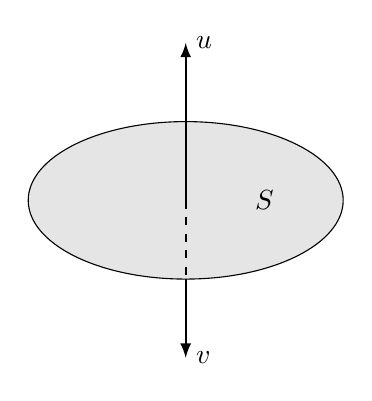
\begin{tikzpicture}
    \draw[fill=gray!20] (0,0) ellipse[x radius=2cm, y radius=1cm];
    \draw[thick, -latex] (0,0) -- ++(0, 2) node[right]{$\vv{u}$ }; 
    \draw[thick, dashed] (0,0) -- ++(0, -1);
    \draw[thick, -latex] (0, -1) -- ++(0, -1) node[right]{$\vv{v}$ }; 
    \draw (1,0) node{$S$ };
  \end{tikzpicture}
  \captionof{figure}{Représentation des deux orientations possibles $\protect\vv{u}$ et $\protect\vv{v}$ de la surface $S$. } 
\end{center}

\subsection{Orientation du contour}%
\label{sub:orientation_du_contour}
le contour d'une surface $S$ orientée est lui-même orienté (on lui donne un sens de parcours) de telle sorte que la surface $S$ se trouve à la gauche d'un observateur qui marche sur le contour de $S$ (avec la normale vers le haut). On peut aussi utiliser la \emph{règle de la mobilette} ou la \emph{règle du tire-bouchon} pour déterminer l'orientation du contour en fonction de l'orientation de la surface.  
\begin{center}
  \begin{tikzpicture}[baseline={(0,0)}]
    \draw[fill=gray!20] (0,0) ellipse[x radius=2cm, y radius=1cm];
    \draw[-{Stealth[width=10pt, length=10pt]}] (0, -1) --++(0.1,0);
    \draw[thick, -latex] (0,0) -- ++(0, 2) node[right]{$\vv{n}$ }; 
    \draw (1,0) node{$S$ };
  \end{tikzpicture}
  \hspace{2cm}
  \begin{tikzpicture}[baseline={(0,0)}]
    \draw[fill=gray!20] (0,0) ellipse[x radius=2cm, y radius=1cm];
    \draw[-{Stealth[width=10pt, length=10pt]}] (0, -1) --++(-0.1,0);
    \draw[thick, dashed] (0,0) -- ++(0, -1);
    \draw[thick, -latex] (0, -1) -- ++(0, -1) node[right]{$\vv{n}$ }; 
    \draw (1,0) node{$S$ };
  \end{tikzpicture}
  \captionof{figure}{Représentation des deux orientations possibles de la surface $S$ et de son contour.} 
\end{center}

\subsection{Flux d'un champ magnétique}%
\label{sub:flux_d_un_champ_magnetique}
Si $S$ est une surface orientée par sa normale $\vv{n}$, le flux de $\vv{B}$ à travers $S$ est 
\begin{eqencadre}
  \phi = \iint_S \vv{B}\cdot\vv{n}\D S
\end{eqencadre}
Pour une surface plane ($\vv{n}$ constant) dans un champ magnétique uniforme ($\vv{B}$ constant), on a 
\begin{equation}
  \phi = \iint_S \vv{B}\cdot \vv{n} \D S =  \vv{B} \cdot\vv{n} \iint_S\D S = \vv{B}\cdot\vv{n}S = BS\cos(\theta )
\end{equation}
où $\theta$ est l'angle entre $\vv{n}$ et $\vv{B}$.  

Intuitivement, le flux de $\vv{B}$ correspond au \emph{débit} du champ magnétique à travers la surface $S$.   
\section{Loi de Faraday}%
\label{sec:loi_de_faraday}

\subsection{Courant induit}%
\label{sub:courant_induit}
Lorsqu'un aimant se déplace à proximité d'une bobine, on observe l'apparition d'un courant électrique dans la bobine. Plus précisément on peut faire les observations suivantes :
\begin{itemize}
  \item Lorsque le pôle nord de l'aimant s'approche de la bobine, flux du champ magnétique à travers la bobine augmente et on observe une courant induit $i$  dans le sens indiqué sur la figure~\ref{fig:induit1}. 
  \begin{center}
    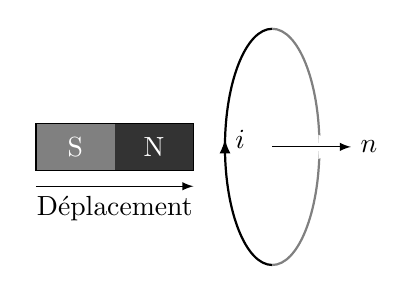
\begin{tikzpicture}
      \fill[gray] (0, -0.3) rectangle (1,0.3);
      \node[white] at (0.5, 0){S};
      \fill[black!80] (1, -0.3) rectangle (2,0.3);
      \node[white] at (1.5, 0){N};
      \draw (0, -0.3) rectangle (2, 0.3);
      \draw[thick] (3,1.5) arc[x radius=0.6cm, y radius=1.5cm, start angle=90, end angle=270];
      \draw[thick, -latex] (2.4, 0) --++(0, +0.1) node[right]{$i$} ;
      \draw[thick, gray] (3,-1.5) arc[x radius=0.6cm, y radius=1.5cm, start angle=-90, end angle=90];
      \draw[-latex] (0, -0.5) -- (2, -0.5)node[midway, below]{Déplacement} ;
      \draw[-latex, preaction={draw, line width=3pt, white}] (3,0) -- ++(1,0) node [right]{$\vv{n}$};  
    \end{tikzpicture}
    \captionof{figure}{Courant induit lorsque le pôle nord de l'aimant s'approche de la bobine.}
    \label{fig:induit1}
  \end{center}
  \item Lorsque l'on éloigne l'aimant de la bobine, on observe que le courant change de sens (figure~\ref{fig:induit2}).
  \begin{center}
    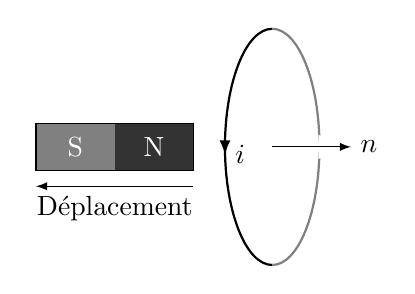
\begin{tikzpicture}
      \fill[gray] (0, -0.3) rectangle (1,0.3);
      \node[white] at (0.5, 0){S};
      \fill[black!80] (1, -0.3) rectangle (2,0.3);
      \node[white] at (1.5, 0){N};
      \draw (0, -0.3) rectangle (2, 0.3);
      \draw[thick] (3,1.5) arc[x radius=0.6cm, y radius=1.5cm, start angle=90, end angle=270];
      \draw[thick, -latex] (2.4, 0) --++(0, -0.1) node[right]{$i$} ;
      \draw[thick, gray] (3,-1.5) arc[x radius=0.6cm, y radius=1.5cm, start angle=-90, end angle=90];
      \draw[-latex] (2, -0.5) -- (0, -0.5)node[midway, below]{Déplacement} ;
      \draw[-latex, preaction={draw, line width=3pt, white}] (3,0) -- ++(1,0) node [right]{$\vv{n}$};  
    \end{tikzpicture}
    \captionof{figure}{Courant induit lorsque le pôle nord de l'aimant s'éloigne de la bobine.}
    \label{fig:induit2}
  \end{center}
\end{itemize}
On en conclut que lorsque le flux du champ magnétique augmente à travers une surface orientée, un courant induit circule dans un sens opposé à l'orientation du contour de la surface. Lorsque le flux du champ magnétique diminue, le courant induit circule dans le sens de l'orientation du contour.

\subsection{Loi de modération de Lenz}%
\label{sub:loi_de_moderation_de_lenz}
Une manière élégante d'exprimer la même observation est que \emph{les effets de l'induction s'opposent aux causes qui l'ont produite}. C'est-à-dire que le courant est induit dans le circuit de telle sorte que le champ magnétique produit s'oppose à la variation de flux qui a produit l'induction du courant. En reprenant l'expérience précédente :
\begin{itemize}
  \item Dans la figure~\ref{fig:induit1}, le flux du champ magnétique à travers la surface de la spire augmente, le courant induit tend à limiter cette augmentation de flux, donc il doit créer un champ magnétique orienté vers la gauche.
  \item Dans la figure~\ref{fig:induit2}, le flux du champ magnétique à travers la surface de la spire diminue, le courant induit tend à limiter cette diminution de flux, donc il doit créer un champ magnétique orienté vers la droite.
\end{itemize}

\subsection{Loi de Faraday}%
\label{sub:loi_de_faraday}
On considère un circuit conducteur $\mathscr{C}$ orienté (arbitrairement) soumis à un champ magnétique $\vv{B}$. Lorsque le flux $\phi$ du champ magnétique à travers le circuit varie, il apparait une force électromotrice (fem) $e$ (orientée dans le même sens que le circuit) telle que 
\begin{eqencadre}
  e = -\dt{\phi}
\end{eqencadre}
C'est la \textbf{loi de Faraday}. 

Si le circuit conducteur possède une résistance $R$, alors le courant induit dans le circuit est $i=\frac{e}{R}$.   

\begin{center}
    \begin{tikzpicture}
      \draw[thick, -latex] (0,0) -- ++(1,0) node[midway, above] {$\vv{B}$}; 
      \draw[thick, postaction={decorate}, decoration={markings, mark= at position 0.3 with{\arrow{latex};}}] (3,1.5) arc[x radius=0.6cm, y radius=1.5cm, start angle=90, end angle=270];
      \draw[thick] (2.4, 0) circle (0.3cm);
      \draw[-latex] (2,0.3) -- ++(0, -0.6) node[midway,left]{$e$}; 
      \draw[thick, gray, ] (3,-1.5) arc[x radius=0.6cm, y radius=1.5cm, start angle=-90, end angle=90];
      \draw[-latex, preaction={draw, line width=3pt, white}] (3,0) -- ++(1,0) node [right]{$\vv{n}$};  
    \end{tikzpicture}
    \captionof{figure}{Orientation du circuit et de la force électromotrice induite pour la loi de Faraday}
    \label{fig:induit1}
  \end{center}
\textbf{Attention, } avant d'appliquer la loi de Faraday, il faut absolument choisir une orientation du circuit, ce qui détermine le signe du flux $\phi$, et le sens de $e$.  
\end{document}
